\cleardoublepage % memastikan bab baru dimulai di halaman ganjil (kanan)
\chapter{PENDAHULUAN}
\label{chap:pendahuluan}
% --- Latar Belakang ---
\section{Latar Belakang}

Instalasi Pengolahan Air atau \textit{Water Treatment Plant} (WTP) merupakan
infrastruktur yang mengolah air baku agar memenuhi standar kualitas sebelum
didistribusikan kepada pengguna. Proses pengolahan secara umum terdiri atas
tahapan koagulasi, sedimentasi, filtrasi, disinfeksi, hingga penyimpanan dan
distribusi air, sebagaimana diilustrasikan pada Gambar~\ref{fig:proses-wtp-umum}.
Salah satu tahapan penting dalam proses tersebut adalah pemberian dosis bahan
kimia, seperti Poly Aluminium Chloride (PAC) untuk proses koagulasi, kaporit
untuk disinfeksi, dan soda ash untuk koreksi pH. Keberhasilan proses tersebut
sangat dipengaruhi oleh kondisi kualitas air baku yang dapat berubah
sewaktu-waktu sehingga pemantauan parameter kualitas air serta proses
pemberian dosis bahan kimia perlu dilakukan secara berkelanjutan. Pemberian
dosis yang berlebihan dapat meningkatkan konsumsi bahan kimia dan biaya
operasional, sedangkan dosis yang terlalu rendah dapat menurunkan efektivitas
proses pengolahan serta menyebabkan kualitas air tidak memenuhi standar yang
ditetapkan.

\begin{figure}[H]
    \centering
    \includegraphics[width=0.7\textwidth]{images/WTP-process.png}
    \caption{Ilustrasi Umum Tahapan Proses \textit{Water Treatment}}
    \label{fig:proses-wtp-umum}
\end{figure}

Pada WTP ITB Jatinangor, proses pemantauan dan pemberian dosis sebelumnya masih
bergantung pada pengoperasian manual, asumsi dosis statis, dan pengamatan
operator. Operator perlu memantau berbagai parameter kualitas air, seperti pH,
kekeruhan, dan \textit{Total Dissolved Solids} (TDS), sekaligus memperhatikan
kondisi pompa dosis dan ketersediaan bahan kimia. Informasi tersebut berasal
dari beberapa sumber yang berbeda sehingga operator harus membandingkan berbagai
instrumen maupun catatan secara terpisah. Kondisi tersebut meningkatkan beban
pemantauan, memperlambat pengambilan keputusan ketika terjadi perubahan
kualitas air baku, serta berpotensi menyebabkan keterlambatan dalam mengenali
kondisi yang memerlukan tindakan.

Berdasarkan tinjauan terhadap jalur perpipaan eksisting WTP ITB Jatinangor
sebagaimana ditunjukkan pada Gambar~\ref{fig:pid-eksisting}, air baku mengalir
dari \textit{Lake} menuju \textit{Pre-Sedimentation Tank}, kemudian diteruskan
ke \textit{Mixing Tank} dan \textit{Extra Tank} sebelum akhirnya disalurkan ke
\textit{Dorm Tank} untuk didistribusikan ke area asrama. Pemberian dosis
kaporit dan PAC pada jalur tersebut (area yang ditandai lingkaran merah) saat
ini sepenuhnya dilakukan secara manual oleh operator: ketika terdapat aliran
air pada jalur pipa, operator menyalakan pompa dosing secara manual, dan
volume dosis yang diberikan ditentukan berdasarkan pengalaman operator tanpa
acuan pengukuran kuantitatif. Titik dosing tersebut belum dilengkapi dengan
sensor analitik maupun sensor konduktivitas untuk memantau kondisi air secara
langsung, serta belum memiliki katup otomatis untuk mengatur aliran bahan
kimia; satu-satunya perangkat yang tersedia adalah pompa dosing yang
dioperasikan secara manual. Kondisi ini menyebabkan proses dosing rentan
terhadap ketidakkonsistenan, bergantung pada kehadiran dan penilaian subjektif
operator, serta tidak memiliki data operasional yang dapat ditelusuri untuk
mendukung evaluasi maupun pengambilan keputusan.

\begin{figure}[H]
    \centering
    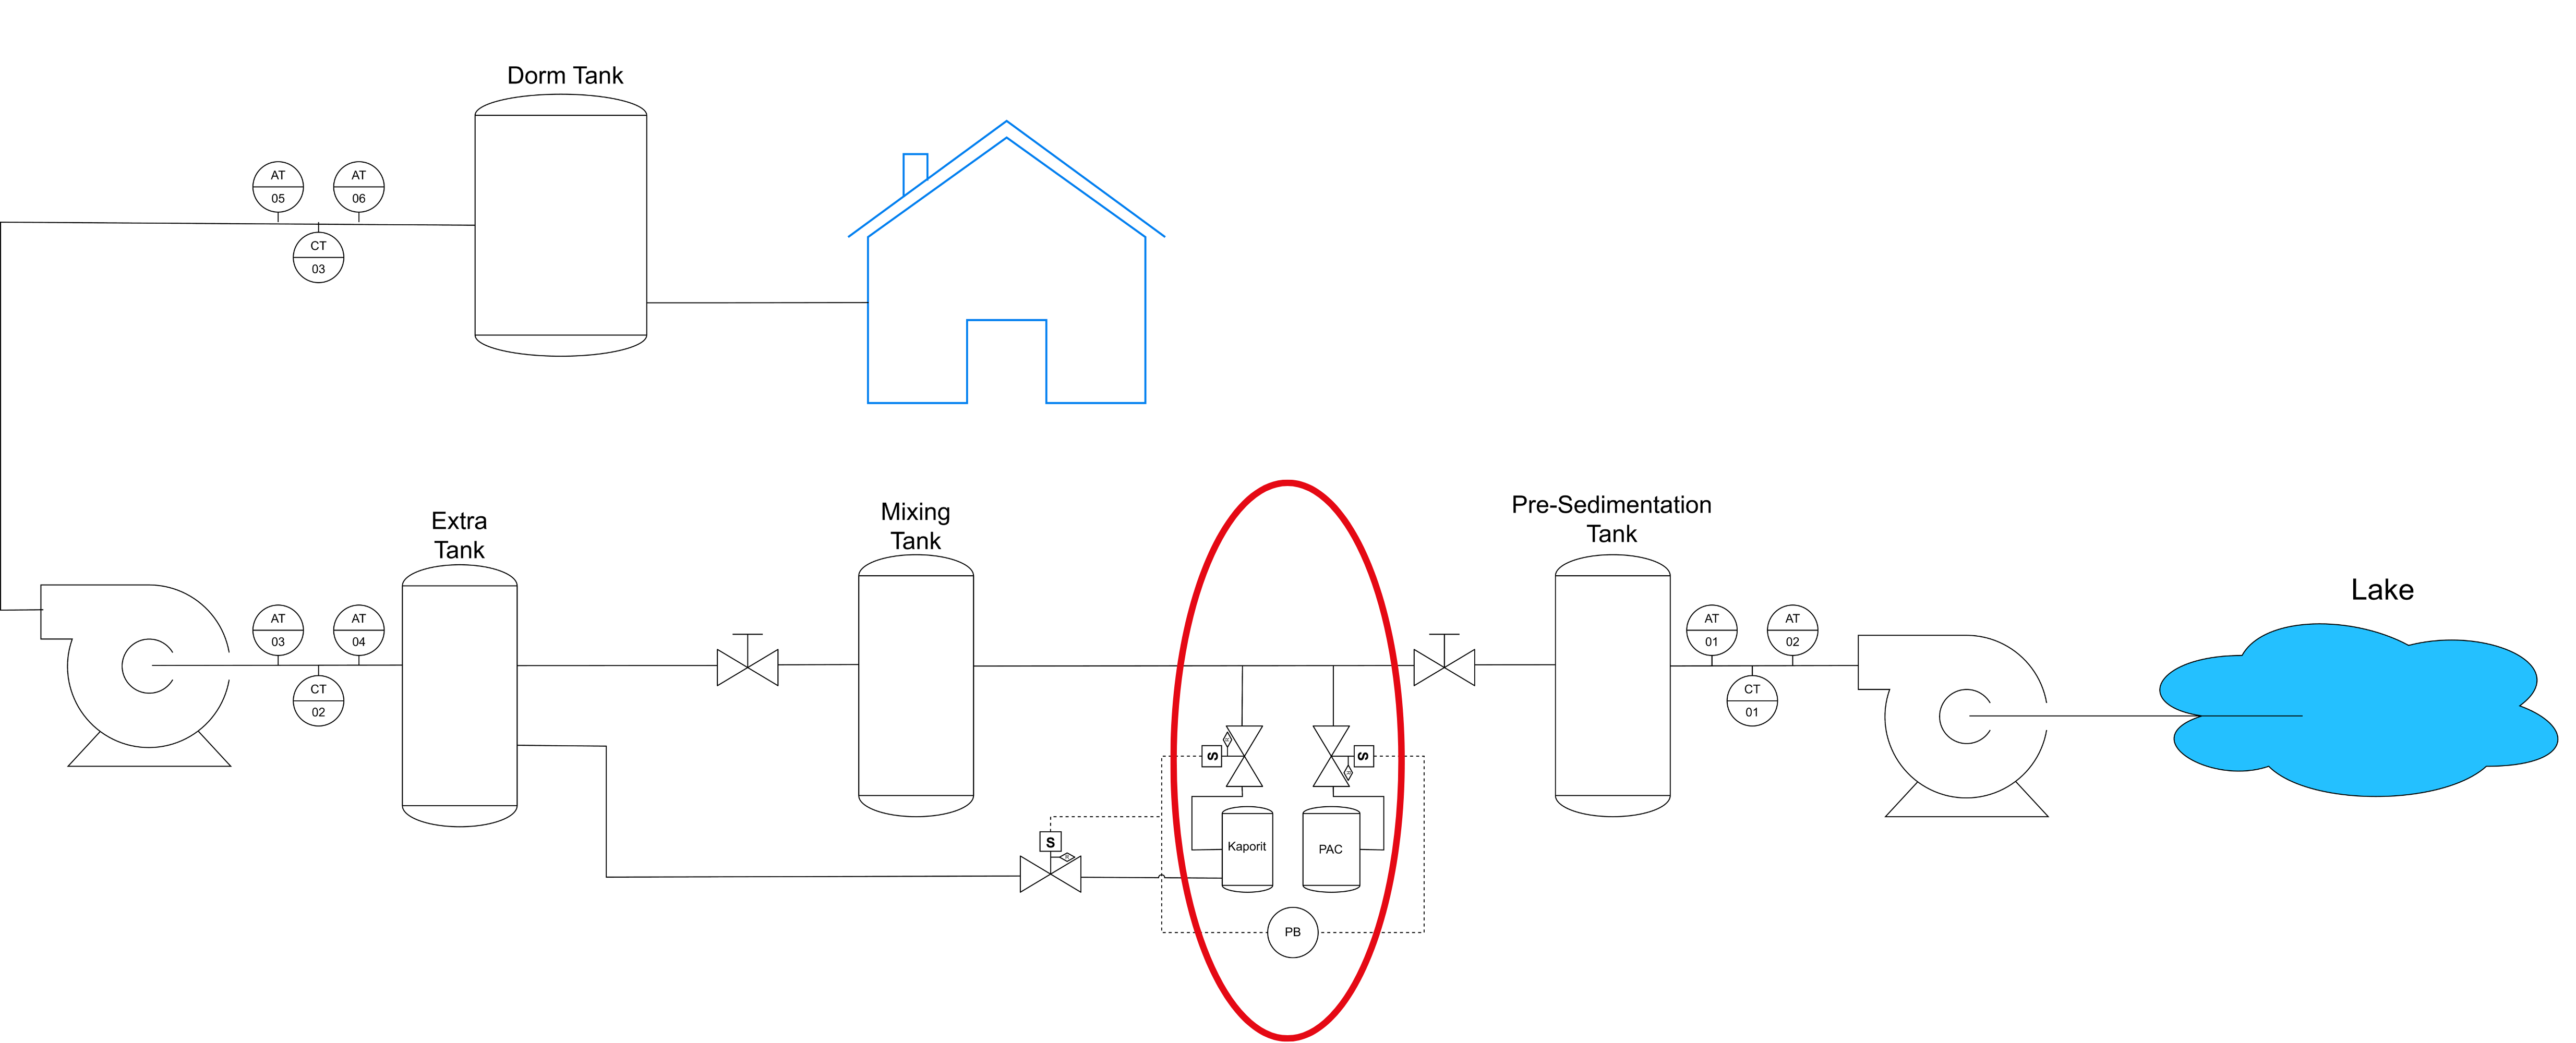
\includegraphics[width=\textwidth]{images/current.png}
    \caption{Diagram Perpipaan Eksisting WTP ITB Jatinangor dengan Titik Otomasi Dosing (Ditandai Lingkaran Merah)}
    \label{fig:pid-eksisting}
\end{figure}

Selain persoalan pada proses dosing itu sendiri, ketersediaan bahan kimia juga
menjadi salah satu aspek penting dalam operasional WTP yang saat ini belum
dipantau secara terpusat.  Operator perlu mengetahui level bahan
kimia yang tersisa pada setiap tangki penyimpanan agar pengisian ulang dapat
direncanakan sebelum bahan kimia habis digunakan. Pemantauan level penyimpanan
bahan kimia yang dilakukan secara terpusat membantu mengurangi risiko
terhentinya proses pemberian dosis akibat keterlambatan pengisian ulang dan
mendukung kelancaran operasional instalasi pengolahan air.

Perkembangan teknologi \textit{Internet of Things} (IoT) memungkinkan data
kualitas air, kondisi perangkat, dan parameter operasional dikumpulkan secara
berkelanjutan dari berbagai sensor \autocite{ismail2022iot}. Penelitian lain
juga menunjukkan penggunaan parameter pH, kekeruhan, dan TDS sebagai indikator
utama dalam sistem pemantauan kualitas air berbasis IoT
\autocite{kumar2024iot}. Pada sisi antarmuka operator, penelitian terdahulu
turut menunjukkan penerapan pemantauan dan kendali berbasis SCADA pada sistem
distribusi air \autocite{low2022scada}, serta penerapan teknologi
\textit{Progressive Web App} untuk mendukung aksesibilitas aplikasi berbasis
web \autocite{azhar2022pwa}. Namun, keberadaan perangkat sensor dan layanan
backend belum sepenuhnya membantu operator apabila informasi yang dihasilkan
belum disajikan melalui antarmuka yang mudah dipahami. Dashboard monitoring
berperan sebagai media yang menyatukan berbagai informasi operasional sehingga
operator dapat memperoleh gambaran kondisi sistem secara menyeluruh, memantau
perubahan parameter secara \textit{real-time}, serta merespons kondisi tidak
normal dengan lebih cepat.

Berdasarkan kondisi tersebut, tugas akhir ini berfokus pada implementasi dan
integrasi frontend dashboard berbasis web untuk sistem otomasi dosis WTP ITB
Jatinangor. \textit{Frontend} dikembangkan menggunakan Next.js, React, dan TypeScript
serta diintegrasikan dengan \textit{backend} melalui REST API. Dashboard menyediakan
ringkasan kepatuhan parameter terhadap standar yang ditetapkan, visualisasi data
sensor, riwayat dan ekspor data, pemantauan alarm, status pompa, informasi
level penyimpanan bahan kimia (\textit{chemical storage}), pengaturan offset
dosis, serta deteksi data kedaluwarsa. Selain itu, aplikasi dirancang sebagai
\textit{Progressive Web App} (PWA) sehingga dapat dipasang dan digunakan pada
perangkat desktop maupun perangkat seluler untuk mendukung fleksibilitas
pemantauan oleh operator.
% --- Rumusan Masalah ---
\section{Rumusan Masalah}
Berdasarkan latar belakang tersebut, persoalan yang dibahas dalam tugas akhir
ini dirumuskan sebagai berikut.
\begin{enumerate}
    \item Informasi kualitas air, level tangki bahan kimia, status pompa
    dosing, dan alarm masih tersebar pada sumber yang terpisah sehingga
    operator perlu memeriksa beberapa instrumen atau catatan yang berbeda
    untuk memperoleh gambaran kondisi sistem secara menyeluruh.
    \item Ketiadaan antarmuka terpusat yang menyajikan status ketersediaan
    bahan kimia dan kondisi pompa dosing secara \textit{real-time}
    meningkatkan risiko keterlambatan operator dalam mengenali kondisi yang
    memerlukan tindakan, seperti tangki bahan kimia yang mendekati habis atau
    pompa yang tidak beroperasi sebagaimana mestinya.
    \item Operator berpotensi mengambil keputusan berdasarkan data yang tidak
    lagi valid apabila antarmuka pemantauan tidak dapat membedakan antara
    data terkini, data yang sedang dimuat, data yang gagal diperoleh, dan
    data yang sudah kedaluwarsa.
\end{enumerate}

% --- Tujuan ---
\section{Tujuan}
Tujuan tugas akhir ini adalah menghasilkan \textit{frontend dashboard} berbasis web yang
terintegrasi dengan sistem otomasi dosis WTP. \textit{Frontend} tersebut diharapkan dapat:
\begin{enumerate}
    \item Menyajikan data pH, kekeruhan, dan TDS terkini maupun historis
    \item Menyajikan ringkasan kepatuhan, level tangki bahan kimia, status pompa,
    dan alarm pada antarmuka operator secara terpusat
    \item Mendukung autentikasi, peninjauan riwayat, ekspor data, pengakuan alarm,
    dan pengiriman offset dosis melalui REST API
    \item Membedakan dan menampilkan status data secara jelas kepada operator,
    baik pada kondisi data sedang dimuat, data kosong, kegagalan pengambilan
    data, maupun data yang telah kedaluwarsa
    \item Memberikan pengalaman penggunaan yang responsif pada perangkat desktop
    dan perangkat seluler
\end{enumerate}

Kriteria keberhasilan tugas akhir ini adalah seluruh kebutuhan fungsional di
atas dapat diverifikasi melalui pengujian fungsional \textit{black-box}
terhadap fitur-fitur \textit{frontend} yang telah diimplementasikan, dengan
hasil pengujian yang dirinci pada Bab~\ref{chap:evaluasi-sistem}.

% --- Batasan Masalah ---
\section{Batasan Masalah}
Ruang lingkup tugas akhir dibatasi sebagai berikut.
\begin{enumerate}
    \item Pekerjaan berfokus pada \textit{frontend dashboard} dan integrasinya mulai dari
    batas REST API sampai antarmuka yang digunakan operator.
    \item Pengembangan perangkat sensor, komunikasi ESP32, MQTT, implementasi
    \textit{backend}, desain basis data, dan algoritma kendali dosis berada di luar ruang
    lingkup.
    \item \textit{Frontend} menggunakan data yang telah diproses dan disediakan oleh
    \textit{backend}; \textit{frontend} tidak melakukan kalibrasi sensor maupun menentukan dosis
    bahan kimia secara mandiri.
    \item Evaluasi difokuskan pada fungsi dan alur interaksi \textit{frontend}, bukan pada
    akurasi sensor, efektivitas proses kimia, atau kinerja algoritma kendali.
    \item Parameter utama yang ditampilkan adalah pH, kekeruhan, dan TDS serta
    informasi operasional PAC, kaporit, dan soda ash.
\end{enumerate}

% --- Metodologi Pengerjaan TA ---
\section{Metodologi}

Pengerjaan tugas akhir dilakukan melalui beberapa tahapan sebagai berikut.

\begin{enumerate}
    \item \textbf{Studi literatur}

    Tahap ini dilakukan untuk mempelajari konsep yang berkaitan dengan instalasi
    pengolahan air (WTP), parameter kualitas air, dashboard monitoring berbasis
    web, serta teknologi frontend yang digunakan, seperti Next.js, TypeScript,
    dan TanStack Query. Studi literatur juga mencakup penelaahan penelitian
    terdahulu sebagai dasar dalam perancangan sistem.

    \item \textbf{Analisis kebutuhan}

    Tahap analisis dilakukan untuk mengidentifikasi kebutuhan sistem berdasarkan
    proses bisnis WTP dan kebutuhan operator. Hasil analisis meliputi identifikasi
    aktor, kebutuhan fungsional dan nonfungsional, alur penggunaan sistem, serta
    data yang dibutuhkan frontend dari backend.

    \item \textbf{Perancangan sistem}

    Berdasarkan hasil analisis kebutuhan, dilakukan perancangan arsitektur
    frontend, struktur halaman, alur navigasi, komponen antarmuka, model
    komunikasi dengan REST API, serta rancangan penanganan berbagai kondisi,
    seperti proses pemuatan data, kegagalan pengambilan data, dan data
    kedaluwarsa.

    \item \textbf{Implementasi dan integrasi}

    Tahap implementasi dilakukan dengan membangun frontend menggunakan Next.js,
    TypeScript, dan berbagai pustaka pendukung. Selanjutnya dilakukan integrasi
    dengan REST API yang disediakan backend sehingga seluruh fitur dashboard dapat
    berfungsi sesuai kebutuhan sistem.

    \item \textbf{Evaluasi}

    Tahap evaluasi dilakukan melalui pengujian fungsional terhadap seluruh fitur
    frontend. Pengujian bertujuan untuk memverifikasi bahwa setiap kebutuhan
    fungsional telah diimplementasikan dengan benar serta seluruh alur interaksi
    aplikasi berjalan sesuai dengan spesifikasi yang telah ditentukan.

    \item \textbf{Penarikan kesimpulan dan saran}

    Tahap akhir dilakukan dengan menarik kesimpulan berdasarkan hasil evaluasi
    terhadap pemenuhan tujuan dan rumusan masalah, serta menyusun saran
    pengembangan lebih lanjut terhadap sub-sistem frontend.
\end{enumerate}

% --- Sistematika Penulisan ---
\section{Sistematika Penulisan}
Laporan tugas akhir ini disusun dalam tujuh bab dengan sistematika sebagai
berikut.
\begin{enumerate}
    \item \textbf{Bab I Pendahuluan}: Berisi latar belakang, rumusan masalah,
    tujuan, batasan masalah, metodologi, dan sistematika penulisan.
    \item \textbf{Bab II Studi Literatur}: Membahas landasan teori dan
    penelitian terkait yang mendukung pengembangan frontend dashboard.
    \item \textbf{Bab III Analisis}: Memuat analisis kondisi, batas sistem,
    serta kebutuhan frontend.
    \item \textbf{Bab IV Perancangan}: Menjelaskan perancangan arsitektur,
    data, komponen, dan antarmuka frontend.
    \item \textbf{Bab V Implementasi}: Membahas implementasi dan integrasi
    frontend dengan backend.
    \item \textbf{Bab VI Evaluasi}: Memuat rancangan serta hasil evaluasi
    fungsional frontend.
    \item \textbf{Bab VII Kesimpulan dan Saran}: Menyajikan kesimpulan dari
    hasil pelaksanaan tugas akhir dan saran untuk pengembangan lebih lanjut.
\end{enumerate}